% Aarav Verma, Engineering Portfolio
% Typeset to match the NOBE X Haylon project paper (Palatino, italic running
% head, numbered sections, booktabs tables).
%
% Build:   cd pdf && tectonic portfolio.tex
% Output:  copy portfolio.pdf to ../public/Aarav_Verma_Portfolio.pdf
%
% Content rules: every claim here comes from src/data/portfolio.ts or the
% current resume. Do not add numbers that are not in one of those.

\documentclass[11pt]{article}

\usepackage[letterpaper,margin=1.05in,headheight=14pt]{geometry}
\usepackage[T1]{fontenc}
\usepackage{newpxtext,newpxmath}
\usepackage{microtype}
\usepackage{graphicx}
\usepackage{xcolor}
\usepackage{booktabs}
\usepackage{tabularx}
\usepackage{array}
\usepackage{enumitem}
\usepackage{fancyhdr}
\usepackage{titlesec}
\usepackage[labelfont=bf,font=small,labelsep=colon]{caption}
\usepackage{subcaption}
\usepackage{siunitx}
\usepackage{float}
\usepackage[hidelinks]{hyperref}

\definecolor{linkink}{HTML}{1F4E79}
\hypersetup{colorlinks=true,urlcolor=linkink,linkcolor=black}

\graphicspath{{figures/}}

% Running head, as in the paper.
\pagestyle{fancy}
\fancyhf{}
\fancyhead[L]{\small\itshape Aarav Verma, Engineering Portfolio}
\fancyhead[R]{\small\itshape November 2026}
\fancyfoot[C]{\small\thepage}
\renewcommand{\headrulewidth}{0.4pt}

\fancypagestyle{plain}{\fancyhf{}\fancyfoot[C]{\small\thepage}\renewcommand{\headrulewidth}{0pt}}

\titleformat{\section}{\Large\bfseries}{\thesection}{0.6em}{}
\titleformat{\subsection}{\large\bfseries}{\thesubsection}{0.6em}{}
\titlespacing*{\section}{0pt}{1.4em}{0.6em}
\titlespacing*{\subsection}{0pt}{1.1em}{0.4em}

\setlist[itemize]{leftmargin=1.4em,itemsep=0.15em,topsep=0.3em}
\setlength{\parindent}{0pt}
\setlength{\parskip}{0.55em}

% A project line: dates on the right, role in italics underneath.
\newcommand{\project}[3]{%
  \par\noindent{\bfseries #1}\hfill{\small #2}\\
  {\itshape #3}\par\vspace{0.2em}}
\newcommand{\tools}[1]{\par{\small\itshape Tools: #1}\par}

\begin{document}

\thispagestyle{plain}

\begin{center}
  {\LARGE\bfseries Aarav Verma\par}
  \vspace{0.35em}
  {\Large\bfseries Engineering Portfolio\par}
  \vspace{0.9em}
  {\itshape B.S. Aerospace Engineering, Minor in Computer Science\par}
  {\itshape University of Illinois Urbana-Champaign\par}
  \vspace{0.7em}
  \href{mailto:aarav.verma.eng0118@gmail.com}{aarav.verma.eng0118@gmail.com}\quad
  (360) 522-0227\quad
  \href{https://verma0118.github.io}{verma0118.github.io}\quad
  \href{https://www.linkedin.com/in/aaravverma0118}{LinkedIn}\quad
  \href{https://github.com/Verma0118}{GitHub}
\end{center}

\vspace{0.6em}
\begin{center}\bfseries Summary\end{center}
\vspace{-0.6em}
\begin{quote}
Aerospace Engineering student at UIUC. I build hardware that flies and moves.
Project Manager at NOBE leading interceptor technology development, and Build
Team Engineer at UAV@Illinois building race-ready FPV drones. This portfolio
collects the current interceptor program, earlier airframe and drivetrain
design work, simulation and analysis studies, and software. Every 3D model
shown here can be turned and inspected on the website.
\end{quote}

% ───────────────────────────────────────────────────────────────────────────
\section{Current Project: Haylon Interceptor UAV}

\project{Haylon Technologies Interceptor Drone}{June 2026 to Present}{NOBE Illinois for Haylon Technologies, Project Manager}

Haylon builds hybrid battery systems for defense and electric aerospace, and
partnered with NOBE on a small interceptor drone. As project manager of six
developers I set the 12-week roadmap, wrote every deliverable and rubric, and
reviewed all CAD and code.

\begin{figure}[H]
  \centering
  \begin{subfigure}[t]{0.32\textwidth}
    \centering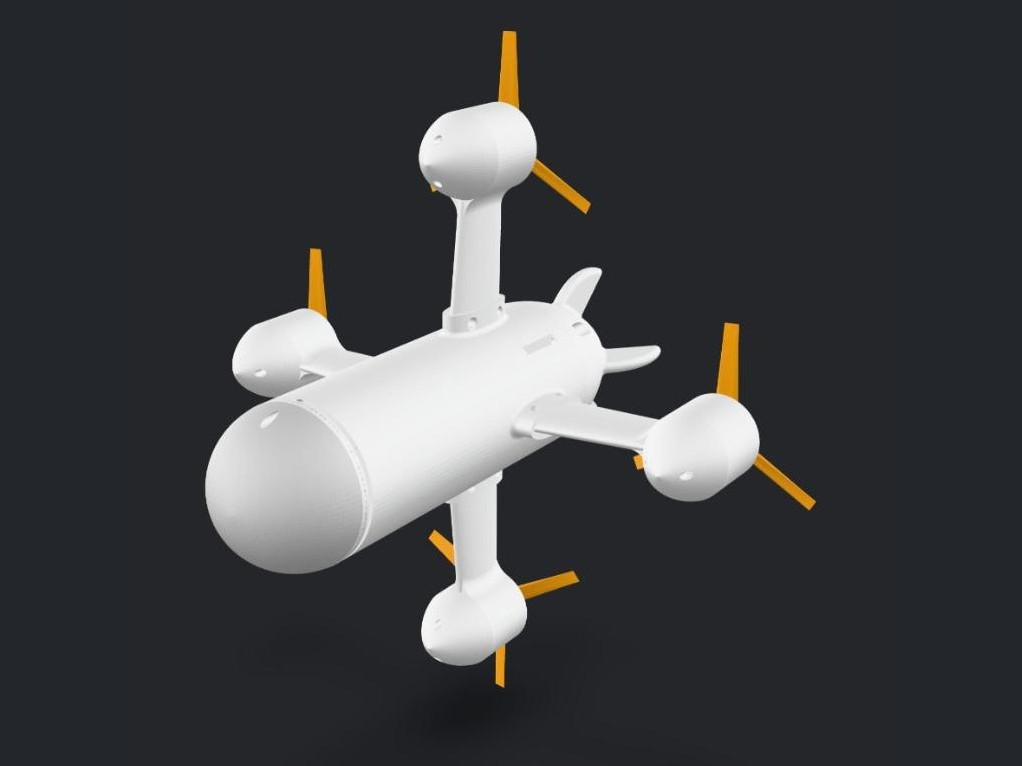
\includegraphics[width=\linewidth]{interceptor.jpg}
    \caption{Interceptor V2 in Fusion 360.}
  \end{subfigure}\hfill
  \begin{subfigure}[t]{0.32\textwidth}
    \centering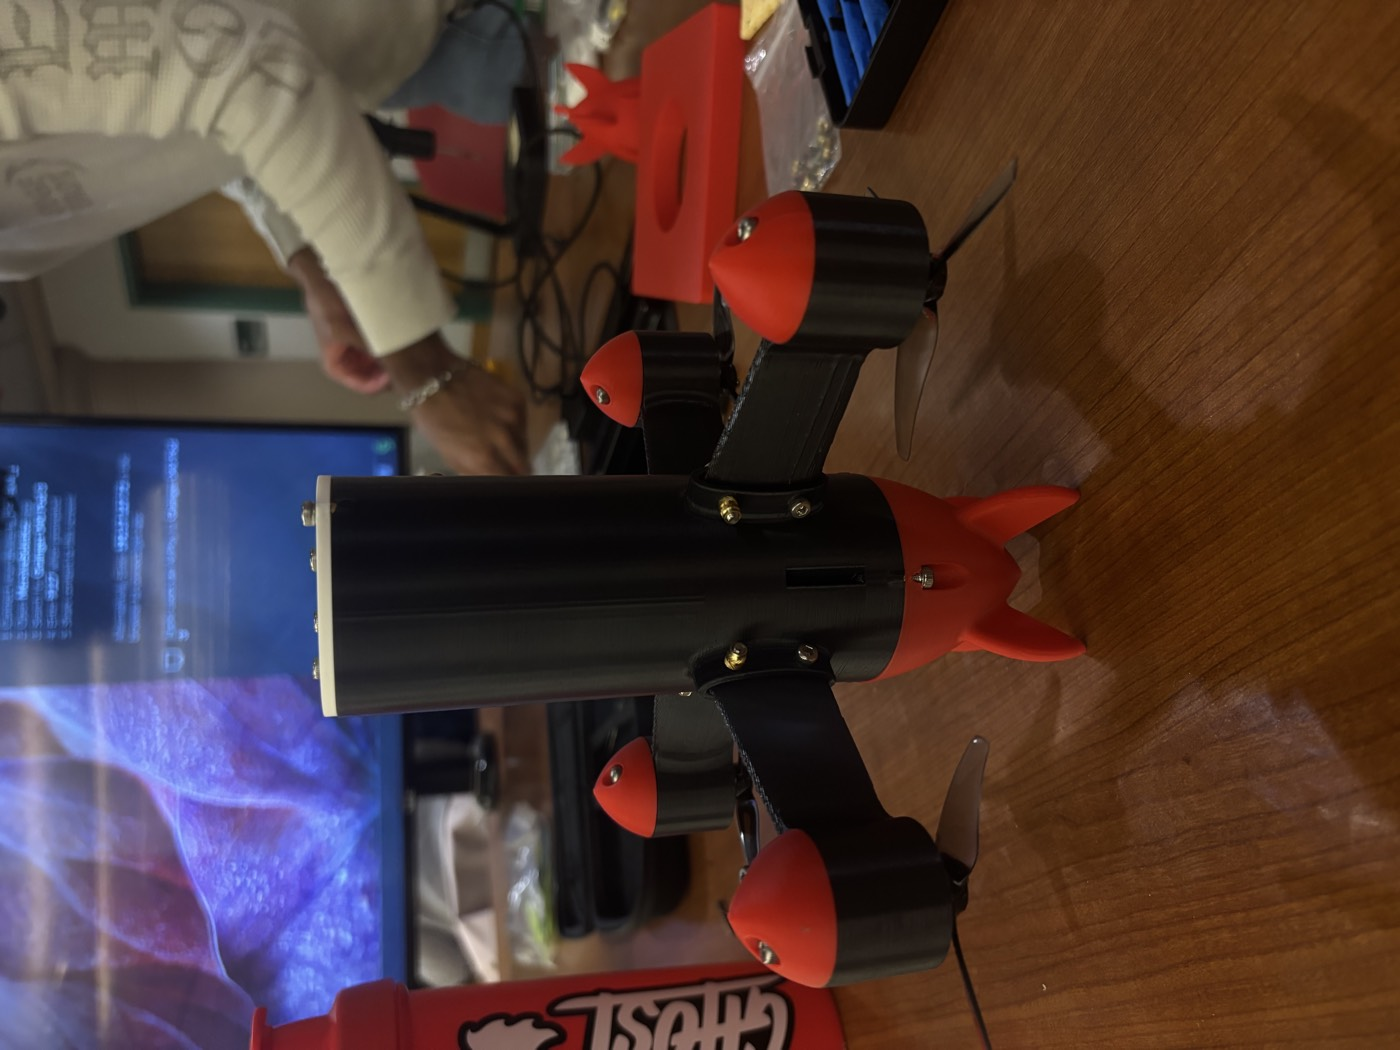
\includegraphics[width=\linewidth,height=0.75\linewidth,keepaspectratio]{assembled-front.jpg}
    \caption{The assembled airframe, Nov 10.}
  \end{subfigure}\hfill
  \begin{subfigure}[t]{0.32\textwidth}
    \centering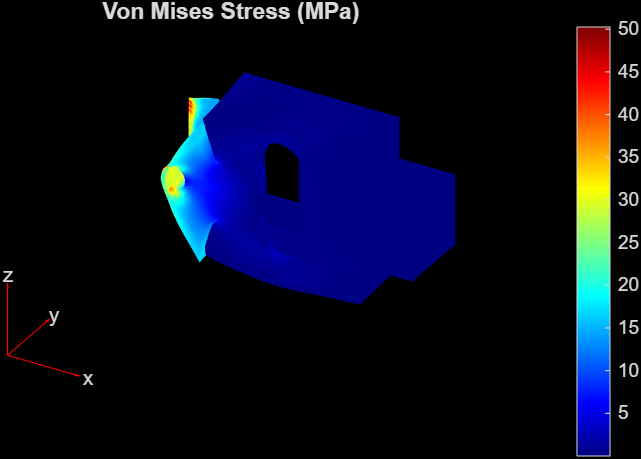
\includegraphics[width=\linewidth,height=0.75\linewidth,keepaspectratio]{camera-stress.png}
    \caption{Camera mount, \SI{35}{m/s} impact.}
  \end{subfigure}
  \caption{Interceptor design, build and analysis.}
\end{figure}

\begin{itemize}
  \item Merged features from a four-way internal design competition into one
        airframe built on M3 heat-set inserts.
  \item Ran two build sessions. The first print exposed three design failures
        and drove a V2 redesign (four-wall winglet adapter, new ESP32 bay); the
        second produced a fully soldered airframe with all four motors seated.
  \item Wrote the FEA deliverable and reviewed all five MATLAB PDE Toolbox part
        studies against a required safety factor of 2.0, catching the camera
        mount at a safety factor of 0.995 under a \SI{35}{m/s} side impact and
        specifying reinforcement before powered flight.
  \item Direct development of a Python vision pipeline (YOLO, ByteTrack) that
        holds persistent tracks with EMA smoothing, ranges targets from a
        calibrated pinhole model, and solves an intercept quadratic for the
        lead point.
\end{itemize}



\begin{table}[H]
  \centering
  \small
  \caption{FEA results summary, PLA at \SI{50}{MPa} yield, required SF 2.0.}
  \begin{tabular}{@{}llrrl@{}}
    \toprule
    Component & Load case & $\sigma_{\max}$ [MPa] & SF & Status \\
    \midrule
    Fuselage body       & Full throttle            & 1.01   & 49.5     & Pass \\
    Electronics plate   & \SI{5}{g} hard landing   & 0.016  & $>2000$  & Pass \\
    Winglet             & Airflow, \SI{35}{m/s}    & 0.0248 & 2013     & Pass \\
    \textbf{Camera mount} & \textbf{Side impact, \SI{35}{m/s}} & \textbf{50.26} & \textbf{0.995} & \textbf{Fail} \\
    Nacelle             & Preliminary traction     & 0.977  & 51.2     & Pass, preliminary \\
    \bottomrule
  \end{tabular}
\end{table}

The full working draft, \emph{NOBE X Haylon Technologies: UAV Interceptor
Project Paper} (22 pages), covers the design competition, both build sessions,
the electronics architecture, and every FEA study in detail:
\href{https://verma0118.github.io/papers/haylon-interceptor-paper.pdf}{verma0118.github.io/papers/haylon-interceptor-paper.pdf}.

% ───────────────────────────────────────────────────────────────────────────
\section{Hardware Design}

\subsection{Canary Drone Project}

\project{Full Drone and Computer System}{Feb 2026 to May 2026}{NOBE, Canary Drone Project, Engineering Lead}
Designed a modular drone airframe in Fusion with a Jetson housing and foldable
leg motors on four snap-lock hinges, with no tools needed to swap
configurations in the field. FEA under a \SI{12}{N} thrust load confirmed a
factor of safety above 2.0, and the BOM covers 50+ components. Presented the
design at the Cozad New Venture Challenge against 300+ teams for \$500,000.
\tools{Autodesk Fusion, FEA, avionics integration}

\project{Toroidal Propeller Design}{Feb 2026 to May 2026}{NOBE, Canary Drone Project, Engineering Lead}
Redesigned a two-blade propeller to a toroidal configuration in Fusion.
Enclosing the blade-tip vortex path raised thrust efficiency about 11\% at
4 to 6k RPM in ANSYS Fluent and dropped the acoustic signature below
\SI{60}{dB} at \SI{1}{m} hover. FEA on the propeller and motor mount under a
\SI{12}{N} load confirmed a factor of safety above 2.0.
\tools{Autodesk Fusion, ANSYS Fluent, FEA, aerodynamics}

\begin{figure}[H]
  \centering
  \begin{subfigure}[t]{0.48\textwidth}
    \centering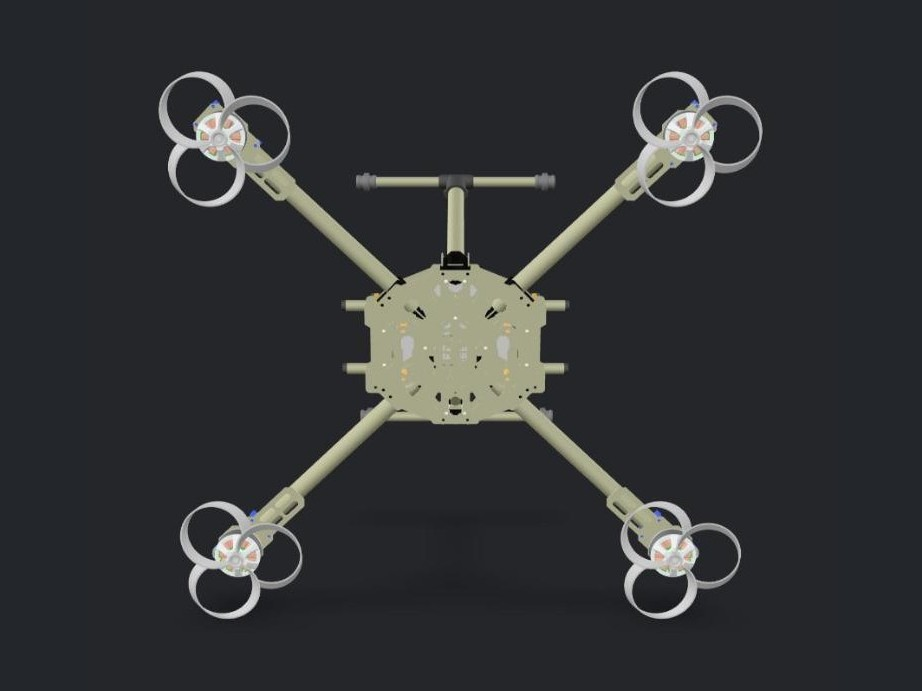
\includegraphics[width=\linewidth]{canary-drone.jpg}
    \caption{Canary airframe with Jetson housing.}
  \end{subfigure}\hfill
  \begin{subfigure}[t]{0.48\textwidth}
    \centering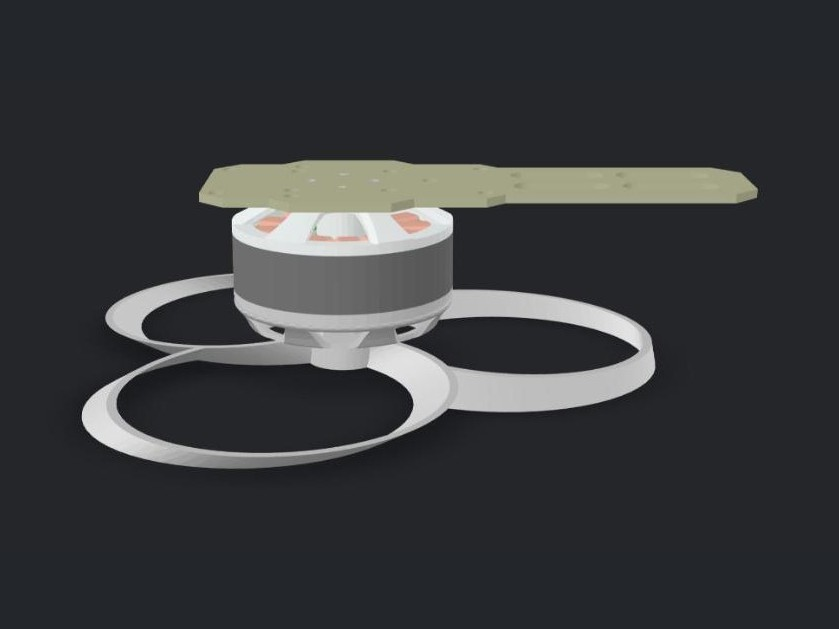
\includegraphics[width=\linewidth]{toroidal-propeller.jpg}
    \caption{Toroidal propeller and motor mount.}
  \end{subfigure}
  \caption{Canary Drone Project models.}
\end{figure}

\subsection{Ghost Electric Motorcycles}

\project{Swingarm Assembly}{Aug 2025 to Jan 2026}{Ghost Electric Motorcycles, Drivetrain Engineer}
Rear suspension swingarm in SolidWorks, reverse-engineered from the 2010
Kawasaki ZX-6R. Worked out anti-squat ratio and pivot geometry to match OEM
kinematics, then validated stiffness under braking, acceleration, and
cornering in ANSYS and MATLAB.
\tools{SolidWorks, ANSYS FEA, MATLAB}

\project{Drivetrain Frame}{Aug 2025 to Jan 2026}{Ghost Electric Motorcycles, Drivetrain Engineer}
Drivetrain frame in SolidWorks to mount and align motor, top rod, and
swingarm to $\pm\SI{0.05}{mm}$. Structural analysis in ANSYS and MATLAB
confirmed stiffness under peak torque, chain tension, and rider weight across
braking, cornering, and full acceleration.
\tools{SolidWorks, ANSYS FEA, MATLAB}

\begin{figure}[H]
  \centering
  \begin{subfigure}[t]{0.32\textwidth}
    \centering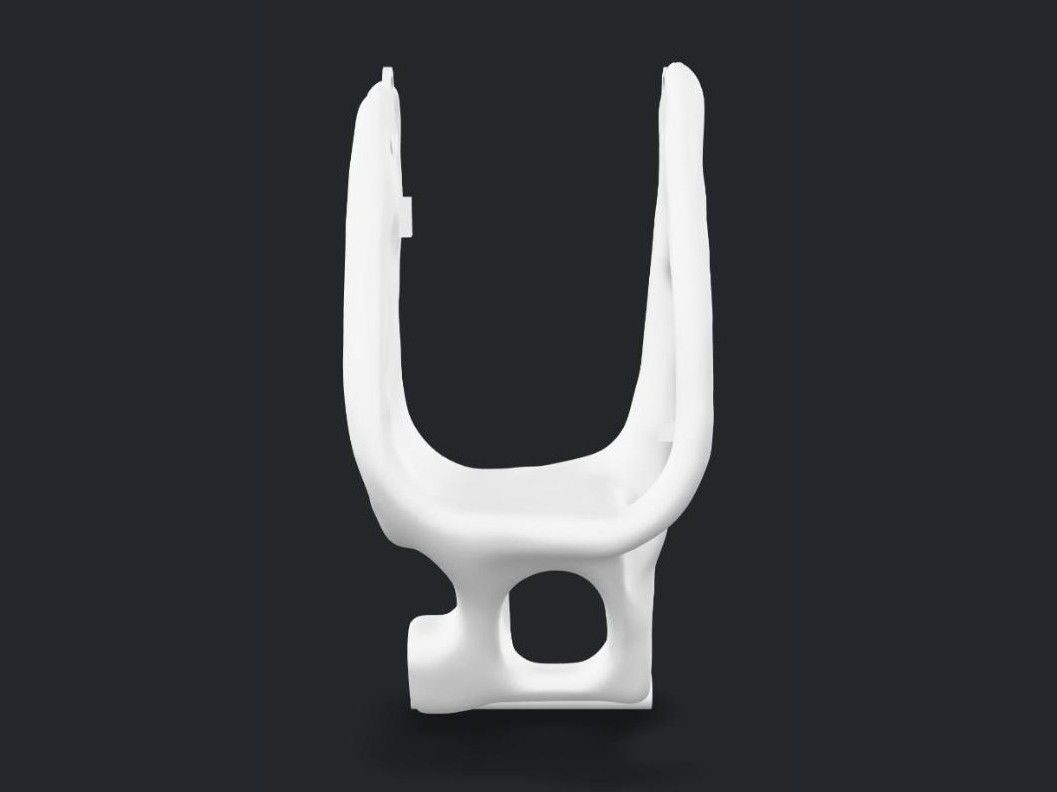
\includegraphics[width=\linewidth]{swingarm.jpg}
    \caption{Swingarm assembly.}
  \end{subfigure}\hfill
  \begin{subfigure}[t]{0.32\textwidth}
    \centering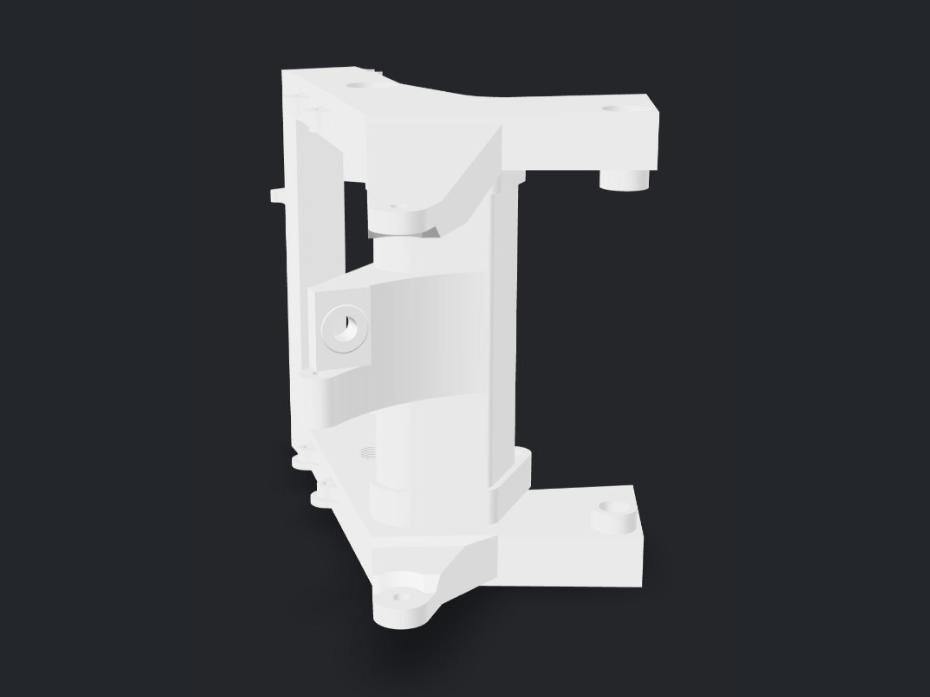
\includegraphics[width=\linewidth]{drivetrain-frame.jpg}
    \caption{Drivetrain frame.}
  \end{subfigure}\hfill
  \begin{subfigure}[t]{0.32\textwidth}
    \centering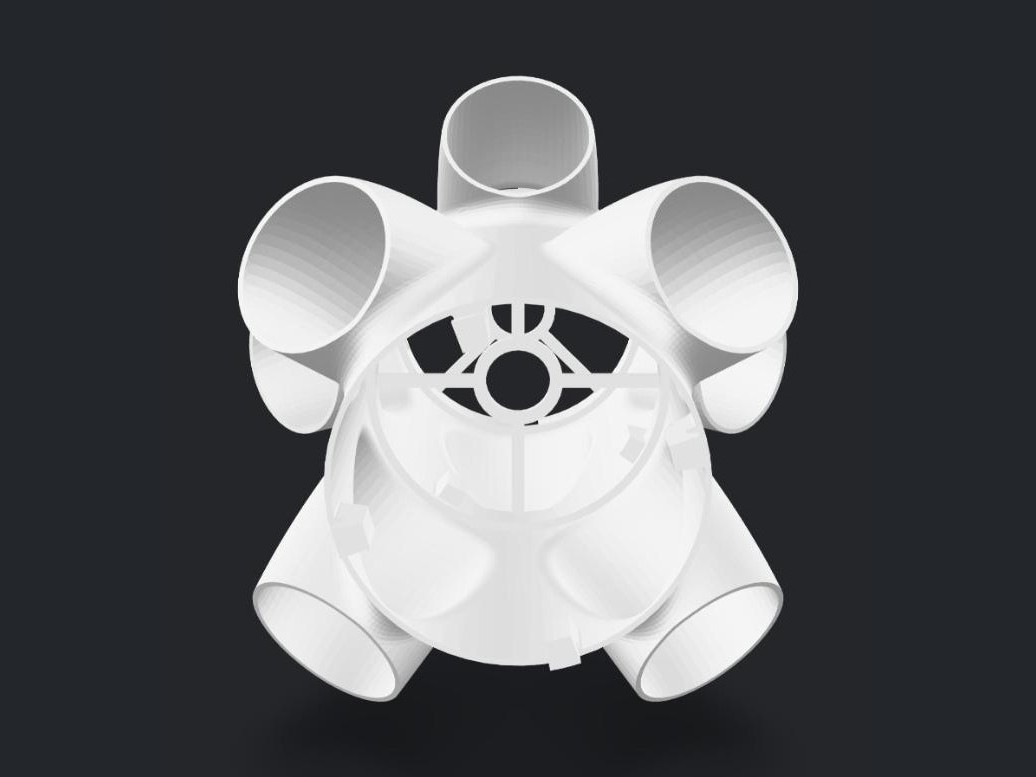
\includegraphics[width=\linewidth]{hydroponic-tower.jpg}
    \caption{Hydroponic tower.}
  \end{subfigure}
  \caption{Drivetrain design for Ghost, and the hydroponic tower prototype.}
\end{figure}

\subsection{Independent Work}

\project{Revolving Modular Hydroponic Tower}{2024}{UIUC Residence Hall Idea Fair, Designer and Builder}
Revolving modular hydroponic tower designed in Fusion. Built the stacking
system around FDM print constraints, with tolerances defined for every
interlocking joint, then printed and assembled the full prototype in-house.
\tools{Autodesk Fusion, 3D printing, DFM}

% ───────────────────────────────────────────────────────────────────────────
\section{Simulation and Analysis}

\project{Actuator-Limited Flight Controller}{Jul 2026 to Sep 2026}{Simulink and controls}
Designed a cascaded rate and angle PID controller (Betaflight and PX4 style)
for a multi-axis UAV model, cutting peak overshoot from 40\% to 10\% by
diagnosing and correcting a derivative-kick and noise-amplification problem.
Characterized actuator saturation and integral anti-windup by sweeping the
motor torque limit, and built a MATLAB 3D visualization pipeline that animates
UAV attitude from logged Simulink flight data.
\tools{Simulink, MATLAB, PID control}

\project{Parametric Airfoil Structural Analysis}{Aug 2026}{MATLAB PDE Toolbox and FEA}
Generated NACA 0012 airfoil geometry in MATLAB, modeled the solid in Fusion,
and imported it into MATLAB for structural FEA under directional aerodynamic
surface loads. A mesh convergence study found a stress singularity at an
unfilleted corner; a CAD fillet brought successive mesh results within 2\% of
each other.
\tools{MATLAB, FEA, Fusion, mesh convergence}

\project{Hand-Validated Cantilever Bracket FEA}{Aug 2026}{MATLAB PDE Toolbox and FEA}
Hand-calculated tip deflection and bending stress before simulating, then
traced a 10x discrepancy between hand calculation and FEA to an incorrect
assumed load-face area, fixed by querying the true face area from the solved
mesh. Reconciled the corrected FEA to within 10\% of hand calculations,
attributing the remaining gap to bend-fillet compliance and hole stress
concentration.
\tools{MATLAB, FEA, mechanics of materials}

\begin{figure}[H]
  \centering
  \begin{subfigure}[t]{0.32\textwidth}
    \centering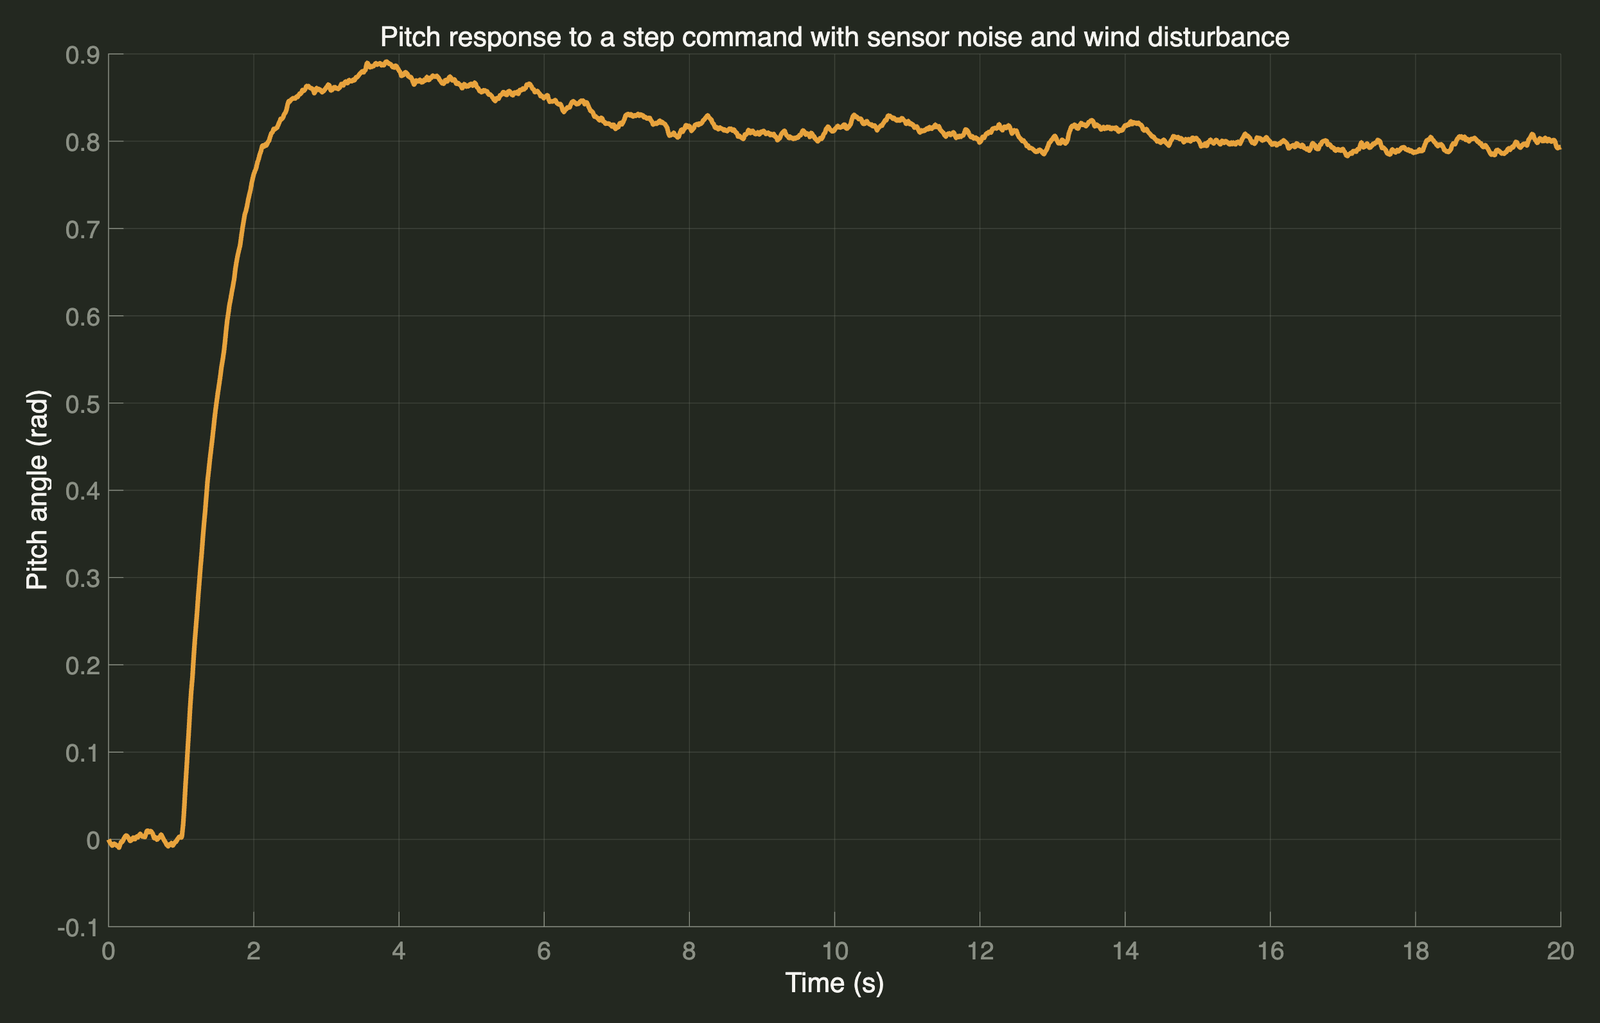
\includegraphics[width=\linewidth,height=0.7\linewidth,keepaspectratio]{simulink-response.png}
    \caption{Pitch response with noise and gust.}
  \end{subfigure}\hfill
  \begin{subfigure}[t]{0.32\textwidth}
    \centering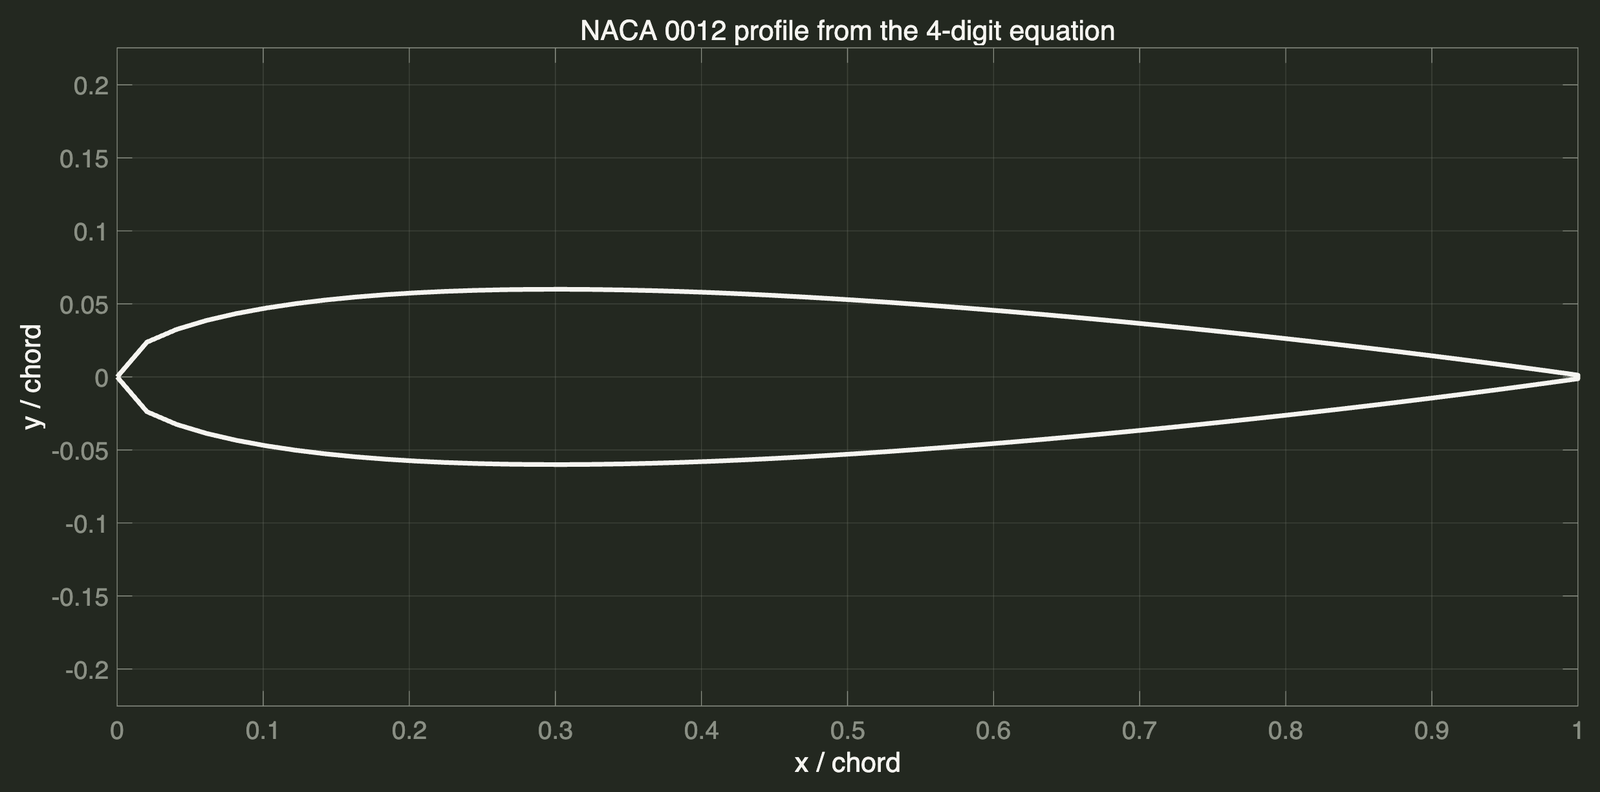
\includegraphics[width=\linewidth,height=0.7\linewidth,keepaspectratio]{airfoil-profile.png}
    \caption{NACA 0012 profile.}
  \end{subfigure}\hfill
  \begin{subfigure}[t]{0.32\textwidth}
    \centering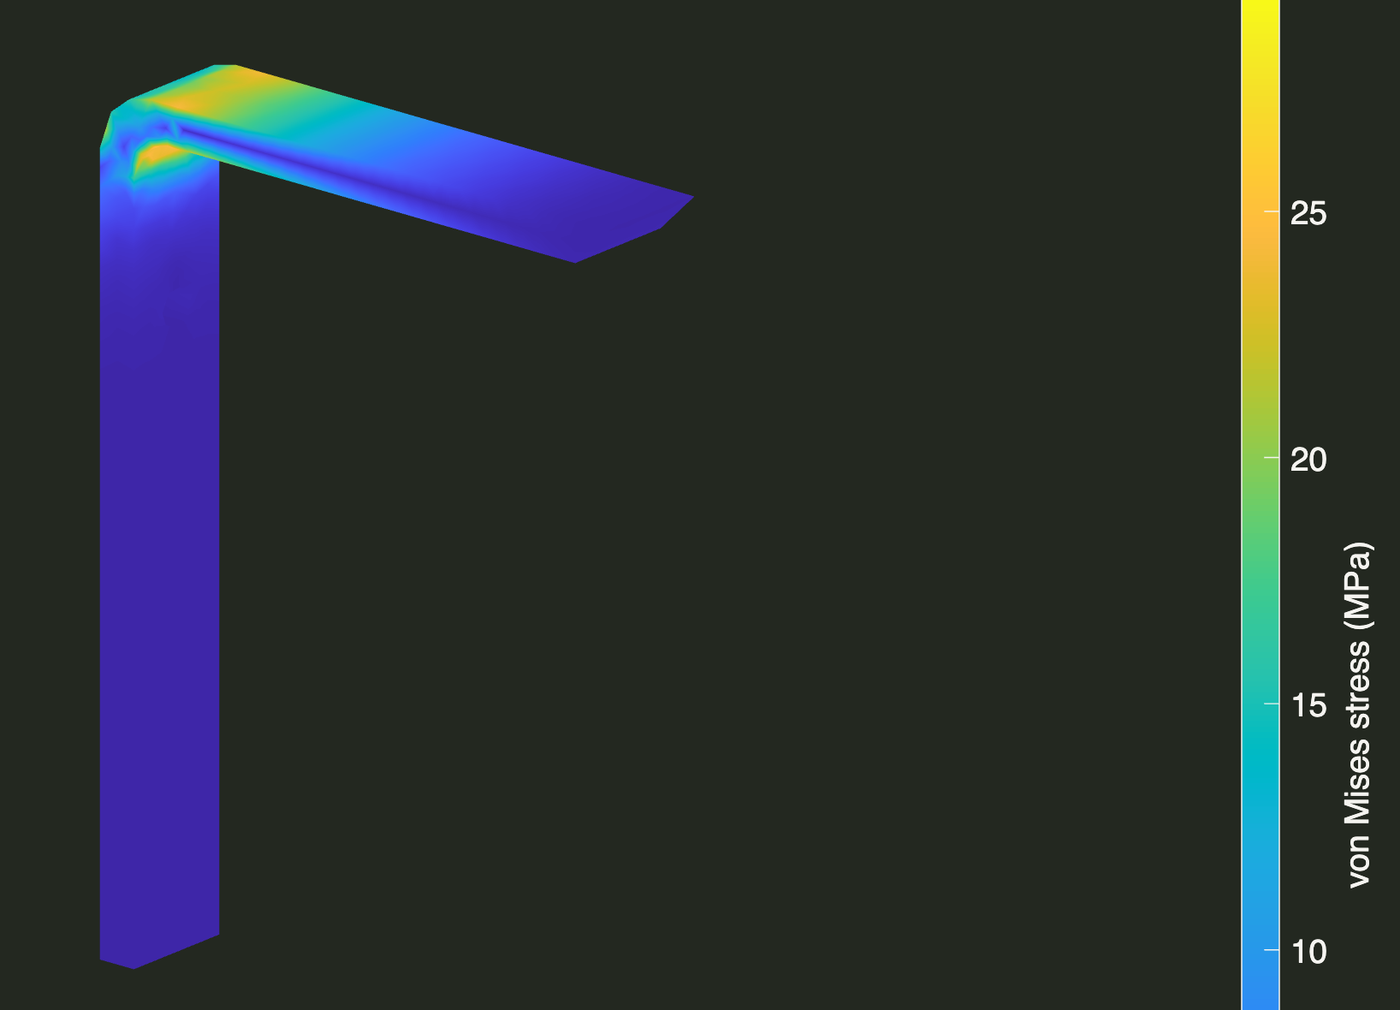
\includegraphics[width=\linewidth,height=0.7\linewidth,keepaspectratio]{cantilever-stress.png}
    \caption{Bracket von Mises stress.}
  \end{subfigure}
  \caption{Simulation and analysis studies.}
\end{figure}

% ───────────────────────────────────────────────────────────────────────────
\section{Software}

\project{Haylon Intercept Sim}{\href{https://github.com/Verma0118/haylon-intercept-sim}{github.com/Verma0118/haylon-intercept-sim}}{Simulation}
A browser simulation of the interceptor's control idea: detect, stabilize,
track, and guide. Throw a target, pick straight, weaving, or erratic evasion,
and watch the guidance law track and chase it in 3D. Built before any CAD or
hardware existed, so the control logic was proven first.
\tools{JavaScript, Three.js, Vite, state machine}

\begin{figure}[H]
  \centering
  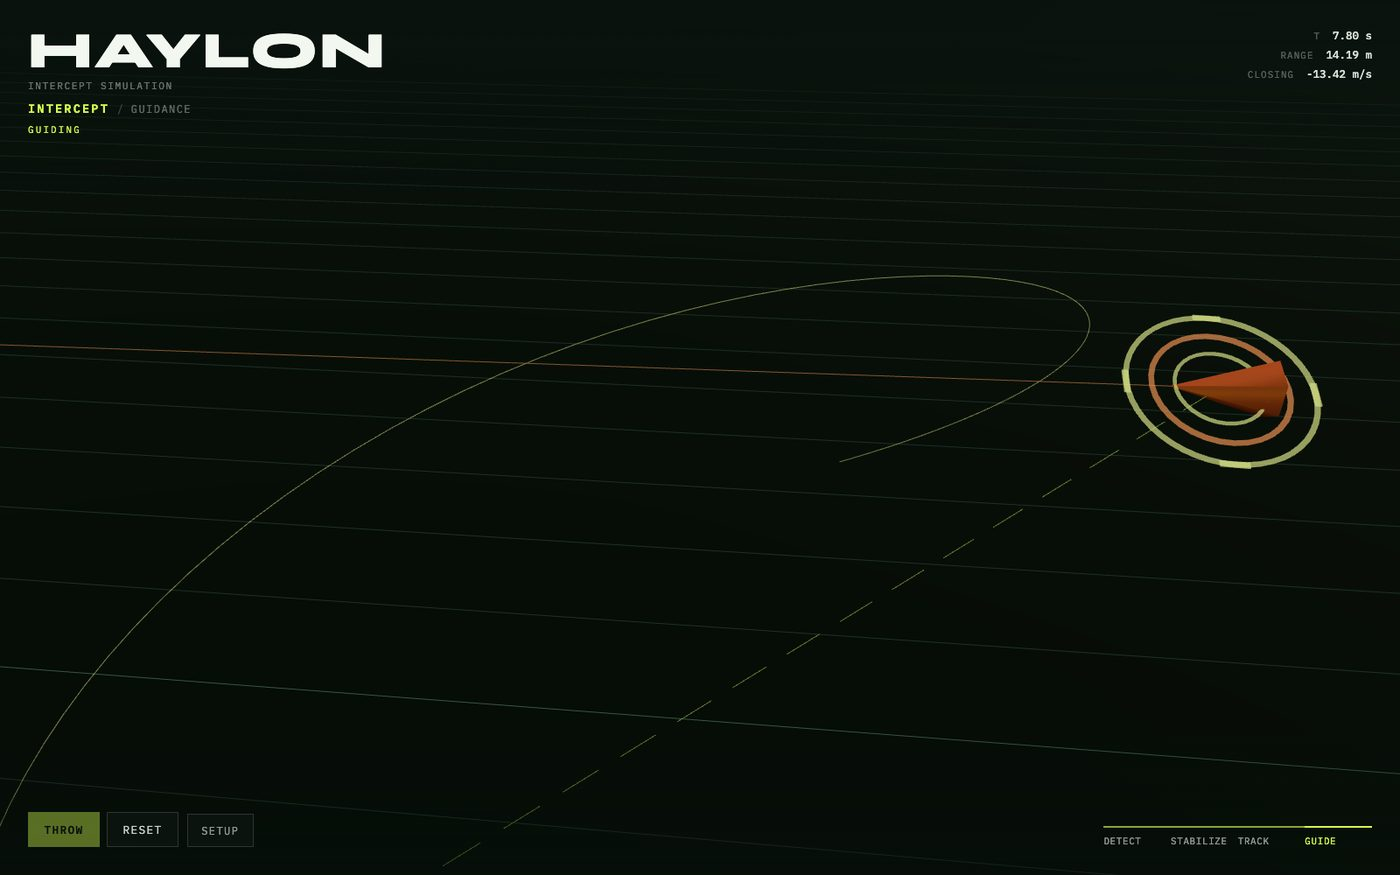
\includegraphics[width=0.62\textwidth]{sim-guidance.jpg}
  \caption{Haylon Intercept Sim during the guidance phase.}
\end{figure}

\project{Volant Compliance Autopilot}{\href{https://volant-compliance.vercel.app/}{volant-compliance.vercel.app}}{Startup}
A drone operator films a walkaround, and Volant turns it into a Part
135-style compliance log. Computer-vision findings and flight telemetry
combine into one verdict: compliant, conditional, or grounded.
\tools{React, TypeScript, computer vision, Vite}

\project{EmailCRM Autopilot}{\href{https://github.com/Verma0118/email-autopilot}{github.com/Verma0118/email-autopilot}}{Automation}
A daily outreach loop that syncs my inbox and drafts replies and cold emails
into an approval queue. Python owns Gmail and the filesystem, Claude handles
judgment, and nothing sends without my approval.
\tools{Python, Gmail API, React, Claude}

\project{TVC Simulator}{\href{https://github.com/Verma0118/TVC_Simulator_V1}{github.com/Verma0118/TVC\_Simulator\_V1}}{Simulation}
Thrust vector control simulator in Python modeling gimbal-actuated rocket
engine dynamics for attitude control during powered flight.
\tools{Python, simulation, controls}

% ───────────────────────────────────────────────────────────────────────────
\section{Experience and Skills}

\begin{table}[H]
  \centering
  \small
  \begin{tabularx}{\textwidth}{@{}>{\bfseries}l X r@{}}
    \toprule
    \multicolumn{1}{@{}l}{Organization} & Role & Dates \\
    \midrule
    NOBE Illinois & Project Manager, Interceptor UAV & June 2026 to present \\
    NOBE Illinois & Engineering Lead, Canary Drone Project & Feb 2026 to May 2026 \\
    Tarform & Mechanical Design Engineer Intern (part-time): production
      drawings and GD\&T per ASME Y14.5 for machined and fabricated
      motorcycle components & Aug 2026 to Oct 2026 \\
    Ghost Electric Motorcycles & Drivetrain Engineer & Aug 2025 to Jan 2026 \\
    UAV@Illinois & Build Team Engineer & \\
    Illinois Space Society & Space Shot Structural Engineer & \\
    \bottomrule
  \end{tabularx}
\end{table}

\begin{table}[H]
  \centering
  \small
  \begin{tabularx}{\textwidth}{@{}>{\bfseries}l X@{}}
    \toprule
    CAD and design & Siemens NX, SolidWorks, Fusion 360, Onshape, CATIA V5, GD\&T (ASME Y14.5), 3D printing (PLA, ABS) \\
    Simulation and analysis & ANSYS FEA, ANSYS Fluent (aerodynamic CFD), MATLAB (PDE Toolbox), Simulink \\
    Programming & MATLAB, Python (NumPy, Matplotlib, OpenCV, YOLO), TypeScript, React, C++, Git, ROS \\
    Manufacturing & FDM 3D printing, CNC machining, laser cutting, sheet metal fabrication \\
    \bottomrule
  \end{tabularx}
\end{table}

\vfill
\begin{center}\small\itshape
Interactive 3D models, build logs and the full FEA write-up:
\href{https://verma0118.github.io}{verma0118.github.io}
\end{center}

\end{document}
